\documentclass[usenames,dvipsnames,tikz]{standalone}
%\usepackage{xcolor}
\colorlet{tBlue}{RoyalBlue!35!Cerulean}
\colorlet{tRed}{Red}
%\usepackage{tikz}
%\usepackage{standalone}
\begin{document}
	
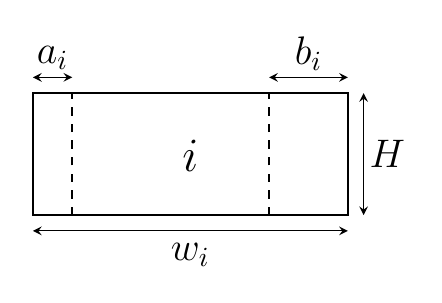
\begin{tikzpicture}
%\draw [help lines] (-1,-2) grid (17,5);

% item i
\draw [thick] (0,0) rectangle (4,1.55);
\draw [thick, dashed] (0.5,0) -- (0.5, 1.55);
\draw [thick, dashed] (3,0) -- (3, 1.55);
\node at (2,0.75) {\LARGE{$i$}};

%arrow and label for width w_i
\draw [<->, >=stealth] (0,-.2) -- (4,-.2);
\node at (2, -.5) {\Large{$w_i$}};

%arrow and label for score width a_i
\draw [<->, >=stealth] (0, 1.75) -- (0.5, 1.75);
\node at (0.25, 2) {\Large{$a_i$}};

%arrow and label for score width b_i
\draw [<->, >=stealth] (3, 1.75) -- (4, 1.75);
\node at (3.5, 2.05) {\Large{$b_i$}};

%arrow and label for height H
\draw [<->, >=stealth] (4.2,0) -- (4.2,1.55);
\node at (4.5,0.775) {\Large{$H$}};

\end{tikzpicture}
	
\end{document}